\documentclass[../main.tex]{subfiles}
\graphicspath{{\subfix{../images/}}}
% Default fixed font does not support bold face
\DeclareFixedFont{\ttb}{T1}{txtt}{bx}{n}{12} % for bold
\DeclareFixedFont{\ttm}{T1}{txtt}{m}{n}{12}  % for normal

% Custom colors
\definecolor{deepblue}{rgb}{0,0,0.5}
\definecolor{deepred}{rgb}{0.6,0,0}
\definecolor{deepgreen}{rgb}{0,0.5,0}


% Python style for highlighting
\newcommand\pythonstyle{\lstset{
language=Python,
basicstyle=\fontsize{10}{10}\selectfont\ttfamily,
morekeywords={self},              % Add keywords here
keywordstyle=\fontsize{10}{10}\selectfont\ttfamily\color{deepblue},
emph={MyClass,__init__},          % Custom highlighting
emphstyle=\ttb\color{deepred},    % Custom highlighting style
stringstyle=\color{deepgreen},
frame=tb,                         % Any extra options here
showstringspaces=false
}}

% Python environment
\lstnewenvironment{python}[1][]
{
\pythonstyle
\lstset{#1}
}
{}

\begin{document}

Se dispone de tres cartas con las características siguientes:
\begin{itemize}
    \item La primera carta es roja por ambos lados.
    \item La segunda carta es verde por ambos lados.
    \item La tercera carta es roja por un lado y verde por el otro lado.
\end{itemize}

Se introducen las tres cartas en una bolsa, se barajan y se extrae una carta completamente al
azar, poníendola sobre la mesa sin mirar y observando posteriormente el lado que ha quedado
visible, el cual ha resultado ser de color verde.

\begin{enumerate}
    \item \textbf{Intuitivamente, ¿cuál crees que es la probabilidad de que al girar la carta el otro lado resulte ser también verde?}
    
    Lo habitual sería responder que la probabilidad es 0.5. La primera intuición nos hace pensar que si el lado visible de la carta seleccionada es de color verde, descartaríamos una de las opciones iniciales (la carta que es roja por ambos lados). Esto nos hace pensar que nuestras probabilidades se centraría en una entre dos opciones, es decir, que al girar la carta o sea verde o sea roja.
    
    Pero este pensamiento inicial lo hacemos sin tomar en consideración que hay una condición previa y que la probabilidad no depende solo de la segunda acción sino que está condicionada por la primera.
    
    Esto lo verificaremos posteriormente en el segundo inciso al hacer una simulación en Python para saber la verdadera probabilidad que resultó ser 2/3
    
    \item \textbf{Realiza una simulación en Python para este problema, estimando la probabilidad tras realizar una cantidad elevada de simulaciones del problema. La función deberá tener como parámetro de entrada el n´umero de simulaciones n y como parámetro de salida una estimación de la probabilidad p. Para simular la extracción de las cartas y del lado visible tras la extracción puedes valerte de \texttt{random.randint}. Recuerda que durante la simulación sólo deberán contabilizarse los experimentos en los que la cara visible de la carta obtenida ha sido verde y, sobre estos, estimar la proporción de veces en las que la carta de la que procede ha resultado ser la que es verde por ambas caras.}
    
    Para corroborar la probabilidad de este problema, se implementó un algoritmo estocástico en Python que al simular la situación N cantidad de veces nos permite aproximarnos de mejor forma a la probabilidad buscada a medida que se incrementa el valor de N. 
    
    \textbf{A pesar de mostrar el código en este documento, el mismo se adjunta en un Jupyter Notebook que se encuentra anexo y donde se puede ejecutar el mismo. }
    
    \newcommand\pythoninline[1]{{\pythonstyle\lstinline!#1!}}
\begin{python}
import random

numero_de_simulaciones = 100000 # Nro de simulaciones que se ejecutarán

def simulacion(numero_de_simulaciones):
    contador_de_exitos = 0
    contador_de_experimentos = 0

    # Definición de las cartas
    cartas = [('roja', 'roja'), ('roja', 'verde'), ('verde', 'verde')]

    for _ in range(numero_de_simulaciones):
        # Se elige una carta de las tres posibles
        carta_de_la_bolsa = cartas[random.randint(0,2)]
        
        # De la carta elegida se toma una de las caras
        cara_visible = carta_de_la_bolsa[random.randint(0,1)]

        if cara_visible == 'verde': # Si la cara es verde se cuenta el experimento
            contador_de_experimentos += 1
            if carta_de_la_bolsa == ('verde', 'verde'): # Si la carta es la verde, verde se cuenta como éxito
                contador_de_exitos += 1
    
    # Se imprime la probabilidad, relación de casos de exito entre casos contabilizados (cara visible verde)
    print(contador_de_exitos/contador_de_experimentos) 

simulacion(numero_de_simulaciones)
\end{python}

El resultado de ejecutar este código y con 100.000 simulaciones resultó en una probabilidad de: 0.6639668826493881
    
    \item \textbf{¿Son los resultados obtenidos consistentes con tu intuición inicial? De no ser el caso, ¿puedes conjeturar el valor correcto de la probabilidad? Una vez realizada, demuestra formalmente que el valor de la probabilidad conjeturada es el correcto y/o proporciona esquemáticamente la explicación de por qué se verifica.}
    
    La simulación evidencia una probabilidad de 2/3 o 0,666666.

Generalmente por intuición descartamos información con la que ya contamos y en este caso es que hay un suceso inicial. Este es un típico ejemplo de Probabilidad Condicionada, donde tenemos que:

P(de que la carta sea la verde, verde) = P(vv) = 1/3, una de tres cartas posibles. P(de que el lado visible de la primera carta sea verde) = P(cv) = 3/6 = 1/2, tres opciones de 6 posibles. P(vv y cv).

Esto podemos esquematizarlo del siguiente modo. Dada la condición de que la cara mostrada ha sido verde, existe la misma probabilidad de 1/3 entre 3 opciones descritas en la tabla de abajo. Que sea la cara verde de la carta verde-roja o que sea algunas de las caras de la carta verde-verde. Al girar y ver la otra cara solo será verde en 2 de 3 casos, es decir 2/3.\\

\end{enumerate}

\centering
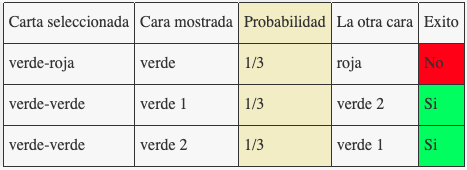
\includegraphics[scale=0.8]{images/table.png}

\bigskip

\end{document}